\documentclass[12pt]{report}
\usepackage{style}

\title{\thesisTitle{}}
\date{\today{}}
\author{Aaron Power}

\makeatletter
\def\@@acrodef{\@ifstar\@acrodefs\@acrodef}
\newtoks\acro@list
\newcommand{\@acrodef}[2]{%
  \global\acro@list=\expandafter{\the\acro@list\@elt{#1}{#2}}%
  \global\@namedef{acro@#1}{n{#1}{#2}}}
\newtoks\acro@resetlist
\newcommand{\@acrodefs}[2]{%
  \global\acro@resetlist=\expandafter{\the\acro@resetlist\@elt{#1}}%
  \@acrodef{#1}{#2}}
\def\acro@doresetlist{\begingroup
  \def\@elt##1{\expandafter\expandafter\expandafter
    \acro@reset\csname acro@##1\endcsname}\the\acro@resetlist\endgroup}
\def\acro@reset#1#2#3{\global\@namedef{acro@#2}{n{#2}{#3}}}
\newcommand{\acro}[1]{\expandafter\expandafter\expandafter
  \use@acro\csname acro@#1\endcsname}
\def\use@acro#1#2#3{\ifx n#1
  #3 (#2)\global\@namedef{acro@#2}{o{#2}{#3}}%
  \else
  #2%
\fi}
\newcommand{\listofacronyms}[1][tabular]{%
  \begingroup\def\@elt##1##2{##1&##2\\}%
  \@ifundefined{chapter}{\section*}{\chapter*}{\listacronymname}
  \noindent\begin{#1}{@{}p{6em}p{\dimexpr\columnwidth-2\tabcolsep-6em\relax}@{}}
    \the\acro@list
  \end{#1}\endgroup}
\providecommand\listacronymname{List of abbreviations}
\newenvironment{acronyms}{\let\acrodef\@@acrodef}{}
\newenvironment{acronyms*}{\let\acrodef\@@acrodef}{\listofacronyms}
\def\g@preto@macro#1#2{\toks0=\expandafter{#1}%
  \toks2={#2}\xdef#1{\the\toks2 \the\toks0 }}
\@ifundefined{chapter}
  {\g@preto@macro\section\acro@doresetlist}
  {\g@preto@macro\chapter\acro@doresetlist}
\makeatother

\begin{document}
  \begin{acronyms}
    \acrodef*{AST}{Abstract Syntax Tree}
    \acrodef*{CSS}{Cascading StyleSheet}
    \acrodef*{HTML}{HyperText Markup Language}
    \acrodef*{I18n}{Internationalization and localization}
    \acrodef*{FFI}{Foreign Function Interface}
    \acrodef*{XSLT}{Extensible Stylesheet Language Transformations}
    \acrodef*{XML}{Extensible Markup Language}
  \end{acronyms}
  \maketitle
  \newpage
  \tableofcontents
  \newpage
  \listoffigures
  \newpage
  \listofacronyms
  \newpage 
  \chapter{Background Research}
  \chapter{Background Research}
\section{Introduction}

A \compiler{}  is a compiler that converts source code into some other form of source code, as opposed to a traditional compiler which converts human readable source code into machine instructions. This has a wide array of uses within different implementations. CMS'(Content Management Systems) have templates that writers pass in their writing to format it into a HTML article on their Website. Academics use \LaTeX{} to convert plain text into scientific documents, and reports. Their use in this thesis is to create a templating language which is a programming language that will convert it's source code into HTML for use in Web applications. The purpose of \languageName{} is to create a templating language that Web developers can use to have more modular, and scalable markup in their Web application.

While there is no definitive first templating language. Their popularity began around the late 1990's with XSLT(Extensible Stylesheet Language Transformations) in 1999 in a W3C recommendation document \parencite{XSLT}. Which was designed for transforming XML(Extensible Markup Language) documents into other formats IE: PDF's as shown in \parencite{XSLTEx}.
\newpage 

One of the most popular modern templating languages for use within Web applications is \parencite{Mustache}. Mustache is a ``\textit{logic-less}'' templating language, meaning it has no explicit control flow statements \textit{if, else, for} according to the \parencite{MustacheMan}. Everything is instead based on the object that is passed to the template See Figure ~\ref{fig:mustacheEx}. So if the developer couldn't change the markup if someone's name started with A instead of B unless they add a key to the hash before they pass it to the Mustache templating engine. Mustache is not a HTML specific templating language. Meaning it's syntax is completely independent from it and can be used with anything. However this also means it as language can't use assumptions based on the language leading the syntax to be very verbose. 

\begin{figure}[ht!]
    \small
    \setstretch{1.0}
    \begin{verbatim}
            A typical Mustache template:

                Hello {{name}}
                You have just won {{value}} dollars!
                {{#in_ca}}
                Well, {{taxed_value}} dollars, after taxes.
                {{/in_ca}}

            Given the following hash:

                {
                  "name": "Chris",
                  "value": 10000,
                  "taxed_value": 10000 - (10000 * 0.4),
                  "in_ca": true
                }

            Will produce the following:

                Hello Chris
                You have just won 10000 dollars!
                Well, 6000.0 dollars, after taxes.
    \end{verbatim}
    \caption{A Mustache Example, from \parencite{MustacheMan}}
    \label{fig:mustacheEx}
\end{figure}
\clearpage



\section{Advantages of a templating language in the Web.}
As the Web has advanced there has always been a need to be able to have the document delivered to the user to be able to be changed based on who, and how the document is being requested. The most popular way to do this currently is to serve the user a nearly blank HTML(HyperText Markup Language) document containing links to JavaScript files that once downloaded, and executed will fill the DOM(Document Object Model) with the data, and information based on the user's request. Prime examples of this is JavaScript frameworks like React. In which the standard is to have a HTML document with a single \textcolor{red}{<div>} element, and let React build the DOM once it can.

%%%%%%%%%%%%%%%%%%%%%%%%%%%%%%%%%%%%%%%%%%%%%%%%
\begin{figure}[ht!]
    \small
    \setstretch{1.0}
    \begin{verbatim}
        <!DOCTYPE html>
        <html>
            <head>
                <meta charset="UTF-8" />
                <title>Hello React!</title>
                <script src="build/react.js"></script>
                <script src="build/react-dom.js"></script>
                <script src="build/script.js"</script>
            </head>
            <body>
                <div id="example"></div>
            </body>
        </html>
    \end{verbatim}
    \caption{Standard React HTML index file}
\end{figure}
%%%%%%%%%%%%%%%%%%%%%%%%%%%%%%%%%%%%%%%%%%%%%%%%

This comes with problems. The content of the Web page is dependent on the JavaScript. While the JavaScript is being downloaded the user will only see a blank page. This problem becomes especially apparent when the user is on a mobile network, or has a slow connection. Studies have shown that 47\% of mobile users expect a site to load in less than two seconds, that 40\% of mobile users will abandon a site if it doesn't load in three seconds or less, and that 52\% of users said that a quick page load is important to site loyalty according to \parencite{MobileLoad}. In large scale applications, and businesses JavaScript size quickly becomes a huge bottleneck in the load times of Websites as shown by \parencite{VergeJS}.\newline

It is in this area in particular that the advantages of using a templating language is seen. With a templating language the content of the Web page can be sent in the initial HTML page, making the ``perceived'' load time of the Web page very quick. Giving the JavaScript more time download than if the user were to see a blank page.\newline

Having a templating language can also provide good separation between the data model of the language, and the design of the page. The designers, or client-side programmers who are formatting the Web page don't have to worry about how the server-side logic works, or write code that could change server's data-model in order to change the format of the Web page. 
\newpage
\section{Main features of \languageName{}}
From doing my own research and looking at the two comparisons of both templating languages in established server-side programming languages(\textit{PHP, C\#, .NET}) from \parencite{WikiCompare}, and templating languages made specifically for use in Isomorphic JavaScript which are generally much younger in their development than their traditional language equivalents as shown in \parencite{JSCompare}.

From looking at these languages I think the main features of \languageName{} is to first have inheritance, and includes, and variables which is to mean that you can write parent markup files which have child markup files which when parsed will include the markup of the parent, that arbitrary \languageName{} files can be inserted into other \languageName{} files, and be able to have data injected within the template respectively. 

One feature that seems to be most absent, or lacking in strong support in most the languages is I18n(\textit{Internationalization and localization}) support. In the modern Web it seems that having poor I18n support is a huge weakness in a templating language for the Web. According to Alexa estimates Google.com's top five countries are as follows United States, India, Japan, Brazil, and Russia. Out of 5 of the top countries only one of those is an English speaking country, and only two of which are Latin based languages. It is important now more than ever to have strong support for other speaking languages.
\newpage
\section{Building a \compiler{}.}
Building \compiler{} is a difficult task. The two primary sources for building a \compiler{} will be Compilers Principles Techniques and Tools (2nd Edition) by \parencite{DragonBook} also known as ``\textit{The Dragon Book}'', and Parsing Techniques - A Practical Guide (2nd Edition) by \parencite{ParseTech}. Since the project is for a \compiler{}, and not a traditional compiler, there is a lot within the sources that won't be used. For example The Dragon Book has chapter's such as ``Run-Time Environments'', and ``Machine-Independent Optimizations'' which don't relate as are output is HTML, and not Machine Code. The syntax, and the features of the language will need to be mostly finalised early within the project to prevent any sort of feature creep, or spending time, and resources on changing the style of the language. Especially aspects like whether to have natural templates, which are templates which are independent of the language, and have a much more verbose language similar to \parencite{Mustache}, or to have a much more terse language, but have it only work for outputting HTML files, like \parencite{Jade}. 

\section{Why Rust?}
There are many reasons that make Rust an great candidate for building a \compiler{}. Rust doesn't have a garbage collector that other languages like Java, or JavaScript. This reduces the runtime overhead of the program giving a significant performance boost, which is important for doing on request compilation of templates on a server. Rust's \textcolor{blue}{char} type is a Unicode scalar value. Meaning Rust can handle non-Latin characters much more easily than languages without IE: JavaScript. Which would be an important feature since the \languageName{} will have strong I18n support. Since rust has such a minimal runtime, it has strong FFI(Foreign Function Interface) support, meaning the \compiler{} can be used in servers written in different languages, without requiring the compiler to be rewritten in that language, and keeping the performance gains from having it built in Rust.
  \chapter{Literature Review}
  % \chapter{Determining how to parse a formal language}

\section{Introduction}
% About how compilers work, three parts. the lit review focus on parsing part

\newpage
\section{Language Parsing Design}

\subsection{Determining how to parse the syntax of a language}

A formal language is defined as a set of strings of symbols for use in situations where a natural language(\emph{English}) isn't suitable eg. Mathematics, and Computer programming. Where each symbol has precise semantic, and syntactic relation to each other. Writing formal grammar rules uses a set of finite ``\emph{productions}''. Productions, are rules that signify substitution of symbols within a string, there are typically three symbols when writing productions in formal grammars.

\begin{description}
    \item[\emph{Terminal Symbols}] Symbols which cannot be substituted any further, examples of this in programming languages are single number digits(0-9), and matematical symbols(\emph{+,-,/,*}). Terminal symbols are commonly represented by lowercase letters.
    
    \item[\emph{Nonterminal Symbols}] Symbols which can be reduced further using productions. For example as in \ref{fig:formalGrammar} $A \rightarrow a\ |\ aA$ is a nonterminal rule, as \emph{A} needs to be substituted into either \emph{a}, or \emph{aA}. Nonterminal symbols frequently are represented by uppercase letters.

    \item[\emph{Start Symbol}] is a special Nonterminal symbol signifying the start of a string. Start symbols are represented by a uppercase S, or with a Uppercase letter with a subscript s eg. $S_s$, in order to signify it is different from a Nonterminal \emph{S} symbol.
\end{description}


Productions rules are used show how a compiler will take strings, and convert them into tokens. The tokens are sorted into a hierarchy that can be used by the next stage of the compiler. The \emph{|}, known as the vertical bar or ``pipe'' symbol is just used to symbolise a grouping of rules applying to the same rule.

\begin{figure}[ht!]
    \begin{align*}
    S_s &\rightarrow AB\ |\ CC \\
    A &\rightarrow a\ |\ aA \\
    B &\rightarrow bc\ |\ bBc \\
    D &\rightarrow ab\ |\ aDb \\
    C &\rightarrow c\ |\ cC \\
    \end{align*}
    \caption{Formal grammar syntax, example from \autocite{ParseTech}}
    \label{fig:formalGrammar}
\end{figure}

\subsection{Chomsky hierarchy within formal languages}

When parsing a string as a way to meaningfully turn the language into meaningful data models, \autocite{Chomsky} talks about the need of structured models, rather than using probabilistic models like Markov Chain. Markov chain is a model where the data model changes from different states, based solely on it's most recent state. \autocite{Chomsky} showcases this with the famous example: \\\\ \centerline{``\emph{Colorless green ideas sleep furiously}''} \\

A sentence which is not a semantically valid sentence, but is grammatically correct. In \autocite{Chomsky} he defined what is now known as \emph{\hierarchy{}}, which defines formal languages into four types(Type 0 - 4). As shown in Figure \ref{fig:Chomsky} each type is a subset of the previous. All of Type 4, can be a Type 3, but not all of Type 3 can be Type 4, so multiple rules can describe the same language depending on it's syntax.
\clearpage
\begin{figure}[h]
    \centerline{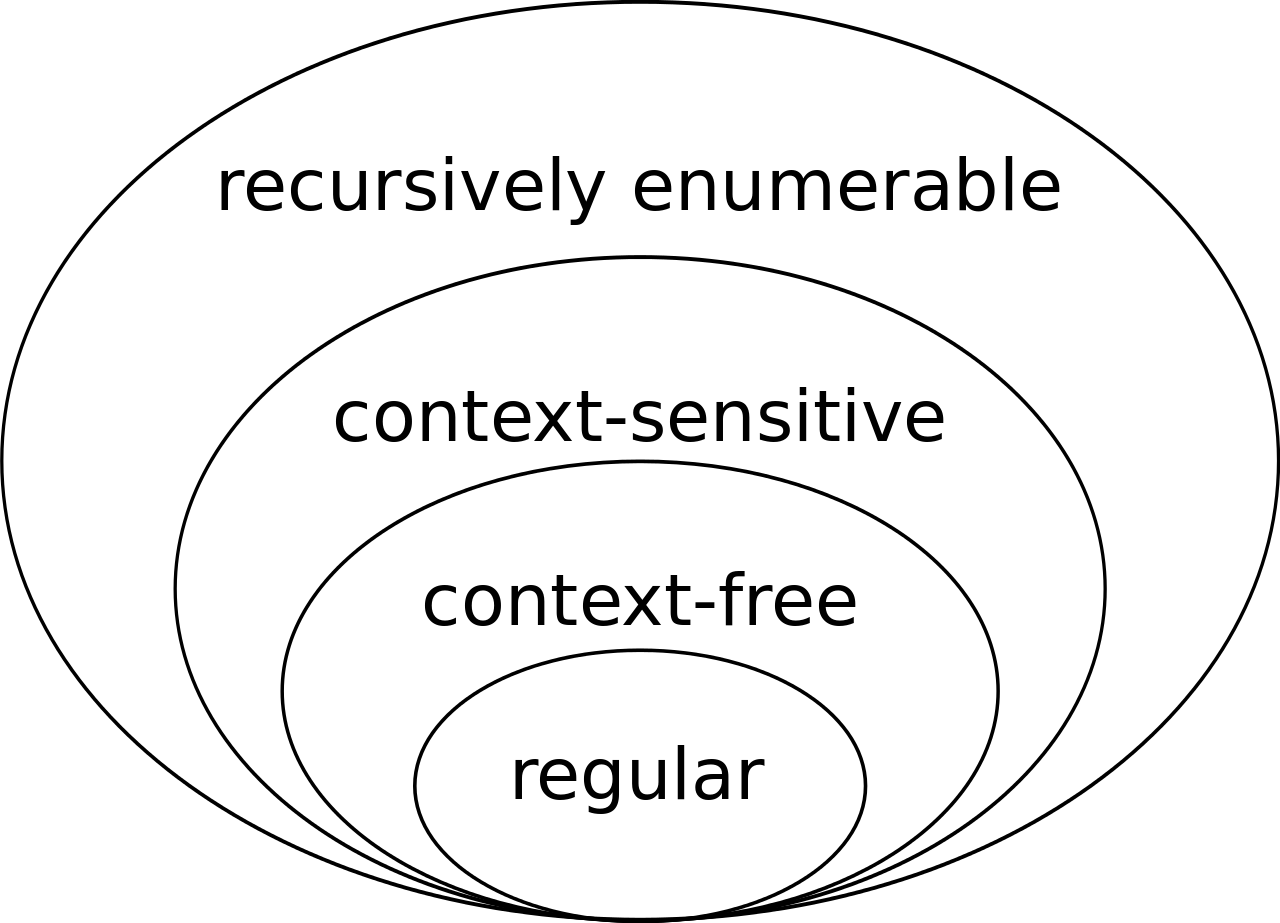
\includegraphics[width=0.5\linewidth]{img/Chomsky.png}}
    \caption{\hierarchy{}, by J. Finkelstein}
    \label{fig:Chomsky}
\end{figure}
\begin{description}
    
    \item[Type 0] Also known as \emph{recursively enumerable} languages. This is the the parent of all following languages. Every language in the Chomsky hierarchy is also a recursively enumerable. Recursively enumerable is a generalised, and can have unclear hierarchy, due to it's lack of limitations.
    
    \item[Type 1] Also known as \emph{context-sensitive} languages. Meaning only one of the nonterminal characters on the left hand side can be replaced. This allows for a much clearer hierarchy within the parse tree.
    
    \item[Type 2] Also known as \emph{context-free} languages. context-free is similar to context sensitive, except there is always only one Nonterminal Symbol on the left hand side. This prevents children in the parse tree to have star patterns with multiple parents pointing to the same child, which then points to multiple children within the parse tree. This is known as a \emph{pure} hierarchy. This is a the language type most programming languages fall under, with few exceptions(\emph{C++}).

    \item[Type 3]  Also known as \emph{regular} languages. Regular languages are languages defined by \emph{regular expressions} rather than regular grammar like seen previously. Regular expressions are often used when the lexical rules of a language are simple, and don't require powerful notations like grammars. Regular expressions are also much more concise in the expressing notation, than it's grammar equivalents. However regular expressions cannot describe nested structures within the language, which can be very limiting \autocite{DragonBook}.
\end{description}

\subsection{Using \hierarchy{} \\within a compiler}
When discussing about parsing a programming language, it is important to differentiate between the syntax of the language, and the \emph{semantics} of the language. As confusion between the two can lead an individual to believe a language is one type, when it is actually a subset. As \autocite{DragonBook} shows, compilers when parsing language have a lexical analyser, which would group characters into much more meaningful sequences known as \emph{lexemes}. Lexemes are then converted into a tokens commonly in the form of a key, value pairing.\\\\ \centerline{(\emph{token-name}, \emph{attribute-value})} \\

Raw symbols like digits, or mathematical symbols(\emph{+,-,/,*}) are mapped into their token-name equivalents. Where as variables, the compiler will map the token-name to a token representing that it is an identifier eg. \emph{id, ident, identifier}. The compiler will then assign the attribute-value to number representing it's key in the Symbol-Table. The Symbol-Table is designed to contain much more concrete information about the token, such as it's name, and it's type eg. \emph{int, float, double, string}. The set of tokens is then passed to the syntax analyser. 

The syntax analyser will only look at the token-name getting only a vary abstract representation of the code, and can only report syntactical errors such as using wrong keywords, or having incorrect mathematically expressions eg $x = 1 + - + 1$. This is shown clearly in Figure \ref{fig:InvalidC}. Where when run through a C compiler the compiler will print out ``\emph{error: \lq{}x\rq{} undeclared (first use in this function)}''. 

\begin{figure}[ht!]
    \begin{verbatim}
                int main() {
                    x++;
                    int x = 1;
                    return 0;
                }
    \end{verbatim}
    \caption{C code with valid syntax, but invalid semantics.}
    \label{fig:InvalidC}
\end{figure}

This could lead an individual that the syntax of the parser, and thus the language must be context-sensitive, as the compiler knew that ``\emph{x}'' was being used before it existed. As seen in \autocite{DragonBook} the compiler could be using a parsing grammar that is context-free, and the semantic analyser is what determined that the code written was invalid. As the syntax analyser goes through each token it builds a parse tree, showing the relationship of the tokens as seen in Figure \ref{fig:AST}. It is solely within the syntax analyser that defines the language type of the programming language.
\begin{figure}[ht!]
    \centering
    \begin{tikzpicture}
        \tikzset{every tree node/.style={align=center,anchor=north}}
        \Tree[.= [.x \textit{id} {} ] 
                 [.+  
                     [.1 ] 
                     [.- {}  
                         [.+ {} 
                             [.1 ] 
                         ] 
                        ]  
                     ]  
                 ]  
             ] 
    \end{tikzpicture}
    \caption{An Abstract Syntax Tree.}
    \label{fig:AST}
\end{figure}

The semantics of the language are typically defined within a semantics analyser. One common part included within the analyser is \emph{type checking}. Where the compiler checks the types on both sides of an operand(\emph{+,-}). An example used in \autocite{DragonBook} is array indexing. As commonly programming languages require the index number to be an integer eg. array[1], not array[1.5].


\autocite{DragonBook} recommends, using a tools like \emph{Lex} for generating code from grammars that were discussed earlier. \autocite{LexYacc} argues that creating parsers like 

\newpage
\section{Conclusion}
\newpage

  \chapter{Practical Guide}
  \section{Introduction}
In this section, the focus will be on constructing \acro{HTML} from Jade, an existing templating language. This example will not cover every feature, or edge case, but will show concisely how a person would build a parser, and how parsing works in practical terms. The Jade that will be converted is the Figure ~\ref{fig:jade}. This will be converted to the code shown in Figure ~\ref{fig:html}, except without the whitespace(except within text), and newlines. The ``->'' character represents the tab character. While Jade can handle tabs or space characters, for simplicity this will focus purely with the tab character. Jade is whitespace sensitive meaning if the the leading whitespace(The whitespace at the start of a line) is more than the previous line, the element on the line is the child of the element from the previous line. The ``.'' syntax as seen in Figure ~\ref{fig:jade}, is shorthand for adding a class to the element so ``\textit{p.article}'' would become ``\textit{<p class=\'article\'></p>}''.

\begin{figure}[ht!]
    \small
    \setstretch{1.0}
    \begin{verbatim}
        html
        ->body
        ->->p.article Hello World!
    \end{verbatim}
    \caption{Sample Jade code to be parsed.}
    \label{fig:jade}
\end{figure}

\begin{figure}[ht!]
    \small
    \setstretch{1.0}
    \begin{verbatim}
        <html>
            <body>
                <p class="article">
                    Hello World!
                </p>
            </body>
        </html>
    \end{verbatim}
    \caption{Sample \acro{HTML} code to be created from Figure ~\ref{fig:jade}.}
    \label{fig:html}
\end{figure}

\section{Definitions}
For this example there will be two main structs(A struct is a basic data structure with fields containing data). The ``\textit{parser}'' struct, and ``\textit{Element}'' struct. Where the parser struct represents the parser itself, and containing methods related to handling the input, and output of the program. Code samples containing method definitions are shorten to signatures for brevity.

\subsection{Element}
The ``\textit{Element}'' struct defines an individual element within both the \acro{AST}, and \acro{HTML}. Markup languages such as \acro{HTML} can usually be translated directly from \acro{AST} representation to code, due to their already present parent-child relation. Features that don't directly translate such as variables, or keywords(extends, includes), it'd be better to have a ``\textit{Node}'' struct, that could contain the either the element struct, or another defining rules of the other features. Both structs also implement the ``\textit{Debug}'' trait to allow them to be easily printed to the console.

\subsubsection{Element Properties}
\begin{itemize}
    \item[\textbf{tag:}] The html tag of the element. eg. \textit{html, body, h1, p}
    \item[\textbf{indentation:}] In Jade leading whitespace defines the hierarchy of the elements. So it is important to keep track of the whitespace.
    \item[\textbf{attributes:}] A Key-Value pairing of the attributes, with the attribute name as the hey, and their value as 
    \item[\textbf{classes:}] The class attribute is the only html attribute that accepts multiple values, so it wouldn't fit within attributes.
    \item[\textbf{text:}] The plain text within the element.
    \item[\textbf{children:}] The child elements of the element.
\end{itemize}

\subsubsection{Element Methods}
\begin{itemize}
    \item[\textbf{new}] Creates, and returns an empty Element.
    \item[\textbf{generate\_html}] Returns a \textit{String} of html code, based on it's properties. This method is also recursive. Calling each of it's children's \textbf{generate\_html} methods.
    \item[\textbf{get \& set}] The get, and set methods for all the properties above.
    \item[\textbf{add \& remove}] For properties containing multiple values like classes, children, and attributes. They would also have methods for pushing, and removing an individual value from them.
\end{itemize}

\begin{figure}[ht!]
    \small
    \setstretch{1.0}
    \begin{verbatim}
      #[derive(Debug)]
      struct Element {
        tag: String,
        indentation: u8,
        classes: Vec<String>,
        attributes: HashMap<String, String>,
        text: String,
        children: Vec<Element>,
      }

      impl Element {
        fn new() -> Self { unimplemented!() }
        fn generate_html(&self) -> String { unimplemented!() }
        fn get_tag(&self) -> String { unimplemented!() }
        fn set_tag(&mut self, tag: String) { unimplemented!() }
        fn get_indentation(&self) -> u8 { unimplemented!() }
        fn set_indentation(&mut self, indentation: u8) 
        { unimplemented!() }
        fn get_classes(&self) -> Vec<String> { unimplemented!() }
        fn set_classes(&mut self) { unimplemented!() }
        fn get_attributes(&self) -> HashMap<String, String> 
        { unimplemented!() }
        fn set_attributes(&mut self) { unimplemented!() }
        fn get_text(&self) -> String { unimplemented!() }
        fn set_text(&mut self, text: String) { unimplemented!() }
        fn get_children(&self) -> Element { unimplemented!() }
        fn set_children(&mut self) { unimplemented!() }
        fn add_child(&mut self, child: Element) { unimplemented!() }
        fn add_attribute(&mut self, key: String, value: String) 
        { unimplemented!() }
        fn add_class(&mut self, class: String) { unimplemented!() }
        fn remove_child(&mut self, child: Element) { unimplemented!() }
        fn remove_attribute(&mut self, key: String) { unimplemented!() }
        fn remove_class(&mut self, class: String) { unimplemented!() }
      }
    \end{verbatim}
    \caption{Element code}
\end{figure}

\subsection{Parser}
The parser struct represents the Parser itself. All logic with regards to moving through the input given by the user is either handled within this struct, or through calling methods on this struct.

\subsubsection{Parser Properties}
\begin{itemize}
    \item[\textbf{input:}] The source code given by the user. Usually the contents of a file.
    \item[\textbf{position:}] The parsers position within the input. 
    \item[\textbf{output:}] A vector of the elements parsed.
\end{itemize}

\subsubsection{Parser Methods}
\begin{itemize}
    
    \item[\textbf{new}] Creates, and returns a new parser containing the source passed in.
    
    \item[\textbf{take}] Returns an Option either containing the next character, and removes it from the input. Or None indicating EOF(End Of File).
    
    \item[\textbf{eof}] checks if we've reached the end of the source.
    
    \item[\textbf{peek}] Returns an Option either containing the next character, but doesn't remove it from the input. Or None indicating EOF.

    \item[\textbf{take\_spaces}] Removes characters until the character isn't whitespace(space, tab, newline, carriage return), and returns how many characters were removed.

    \item[\textbf{take\_until}] Takes, and remove characters from the source until it reaches the character passed as a parameter. Then returns a Result either containing a String of all the characters taken excluding the character passed, or a ParseError indicating that something went wrong while taking the characters. eg. EOF.

    \item[\textbf{peek\_until}] Takes, but doesn't remove characters from the source until it reaches the character passed as a parameter. Then returns a Result either containing a String of all the characters taken excluding the character passed, or a ParseError indicating that something went wrong while taking the characters. eg. EOF.
    
    \item[\textbf{take\_while}] Takes, and removes characters, while the function passed evaluates to false. The function passed in, is passed a char, which is the the latest character in the stream.
    
    \item[\textbf{get \& set}] The get, and set methods for all the properties above.
\end{itemize}

\begin{figure}[ht!]
    \small
    \setstretch{1.0}
  \begin{verbatim}
    #[derive(Debug)]
    enum ParseError {
      EOF,
      EncodingError,
    }
    #[derive(Debug)]
    struct Parser {
      input: String,
      position: usize,
      output: Vec<Element>
    }
    impl Parser {
      fn new(source: String) -> Self { unimplemented!() }
      fn take(&mut self) -> Option<char> { unimplemented!() }
      fn peek(&mut self) -> Option<char> { unimplemented!() }
      fn eof(&self) -> bool { unimplemented!() }
      fn take_spaces(&mut self) -> u8 { unimplemented!() }
      fn take_until(&mut self, character: char) 
      -> Result<String, ParseError> { unimplemented!() }
      fn peek_until(&mut self, character: char) 
      -> Result<String, ParseError> { unimplemented!() }
      fn take_while<F>(&mut self, condition: F) 
      -> Result<String, ParseError> 
        where F : Fn(char) -> bool { unimplemented!() }
      fn get_input(&self) -> String { unimplemented!() }
      fn set_input(&mut self, input: String) { unimplemented!() }
      fn get_position(&self) -> usize { unimplemented!() }
      fn set_position(&mut self, position: usize) { unimplemented!() }
      fn get_output(&self) -> Element { unimplemented!() }
      fn set_output(&mut self, output: Element) { unimplemented!() }
    }
  \end{verbatim}
  \caption{Parser code}
\end{figure}
\newpage
\newpage
\section{Parser Logic}
Once, the program has read the source into memory, and the parser is instantiated the program begins a loop that will run until the end of the source. This loop will contain the logic for parsing. First the program checks if the line is empty or contains all whitespace, if does the program will simply ignore it. Jade is a line sensitive language, so elements can't continue onto the next line without the use of special characters, and their implementation is out of scope for this guide. A new blank element is created, and the parser reads in how many leading spaces on the line in order to determine heirarchy, the heirarchy is defined once every element has been parsed, for simplicity. The program runs the the \textbf{take\_while}, with a closure, that evaluates based on whether the character is a ``\textit{.}'', ``\textit{\#}'', ``\textit{(}'' symbols, or if it is whitespace. For example with the line ``\textit{article.class}'' take\_while will pull out the ``article'', and place that as the element's tag. The program then begins another while loop that continues until the end of the line. Matching for the symbols mentioning before, with ``\#'' meaning id, ``.'' meaning class, ``('' meaning atrributes eg. ``(href=\textquotedbl{}\#\textquotedbl{} required=\textquotedbl{}true\textquotedbl{} style=\textquotedbl{}margin-top: 2px\textquotedbl{})'', and if we find any whitespace everything up to the end of the line is parsed as plaintext. This continues iteraviely until the source is delepted, and the tree of elements is created.


\begin{figure}[ht!]
    \small
    \setstretch{1.0}
  \begin{verbatim}
  use std::io::Read;
  use std::fs::File;
  use std::collections::HashMap;

  fn main() {
    let mut file = File::open("./test.jade").unwrap();

    let mut contents = String::new();
    let _ = file.read_to_string(&mut contents).unwrap();

    let mut parser = Parser::new(contents);

    while !parser.eof() {
      let line = parser.peek_until('\n').unwrap();
      if is_all_whitespace(line) {
        parser.take_until('\n');
        continue;
      }
      let mut element = Element::new();

      element.set_indentation(parser.consume_whitespace());

      let is_not_alphanumeric = |character: char| -> bool {
        !character.is_whitespace() && 
        character != '.' &&
        character != '#' &&
        character != '('
      };

      let tag = parser.take_while(&is_not_alphanumeric);

      element.set_tag(tag.unwrap());
      // continued on next page...        
  \end{verbatim}
  \caption{Program Code. Part 1}
\end{figure}

\begin{figure}[ht!]
    \small
    \setstretch{1.0}
  \begin{verbatim}
      while parser.peek() != Some('\n') {
        match parser.take().unwrap() {
          '.' => {
           let class_name = parser.take_while(&is_not_alphanumeric);
           element.add_class(class_name.unwrap());
           },
           '#' => {
            let id_name = parser.take_while(&is_not_alphanumeric);
            element.add_attribute(String::from("id"), id_name.unwrap());
          },
          '(' => {
            let attributes = parser.take_until(')');
            let attributes:String = attributes.unwrap()
                                              .split_whitespace()
                                              .collect();

            let attributes:Vec<&str> = attributes.split("=")
                                                 .collect();
            for chunk in attributes.chunks(2) {
              let key = String::from(chunk[0]);
              let value = String::from(&chunk[1][1..chunk[1].len()]);
              element.add_attribute(key, value);
            }
          },
          ' ' => {
            element.set_text(parser.take_until('\n').unwrap());
          },
          _ => unreachable!(),
        }
      }
      let _ = parser.take();
    }
  }
  fn is_all_whitespace(string: String) -> bool {
    for character in string.chars() {
      if !character.is_whitespace() {
        return false
      }
    }
    true
  }
  \end{verbatim}
  \caption{Program Code. Part 2}
\end{figure}
  \chapter{Syntax}
  \section{Analysis of other markup languages}

\subsection{Introduction}

In order to decide the syntax of a \acro{HTML} markup language, it is important to examine previous languages, and build on top of their strengths, and try and address their weaknesses. The three main sources used are Jade, a templating built for Node.JS\cite{Jade}, Handlebars.js, a templating language originally built in JavaScript, and has been ported to various other languages, and finally \LaTeX{}, which while not a web markup language, has been in use since 1985\cite{LaTeX}, and thus has a lot more maturity in it's syntax decisions. In addition to research into markup languages, research was done looking into articles written about templating languages by it's users, especially articles that were against the use of templating languages, as it's important to understand templating languages within a larger context, and whether they solve what they set to solve\cite{AgainstTemplating}\cite{LinkedinTemplating}. The main goal of \languageName{}, and it's syntax, is to show a clear, concise, and consistent language providing separation of logic that dictates the form, from content.

\subsection{Jade}

Unlike handlebars, Jade features syntactic sugar for writing html. Jade removes explicit tags, and instead relies on whitespace to determine hierarchy. This allows it to be very terse, lightweight, and simple. A basic example is seen in Figure~\ref{fig:JadeHelloWorld}. However its whitespace dependency can lead to a lot of cases where it's syntax starts to become a hindrance. A simple example of this is shown in Figure~\ref{fig:JadeProblem} where you have paragraph with ``Hello World!'', and within the paragraph the ``World!'' is underlined, and the ``!'' is in bold. This example is arbitrary, but it shows Jade's problems with handling text. Another distinct example of Jade's problem with text is how it handles multi line text, shown in Figure~\ref{fig:JadeMultiLine}. 

Jade assumes the first word in a given line is the name of the element. This resulted in a special character to allow for multi line text, but this can lead to weird indentation to use inline text elements. While \you{} can write normal html elements in the text elements, this solution however leads to inconsistency in the syntax. Even with those two solutions \you{} would still have to make sure that if there is a newline character, that it maintains the same level of indentation. With Jade you have to conform to it's style, rather than have an ideal format suiting to the content. Jade's control flow statements are for the most part the same as JavaScript. Which in the context of being a templating on top of a JavaScript engine, but the file also contained html to solve the previous problem, leads to a file containing three different syntaxes in an attempt to solve the problem of separating logic from content, and in reality only moves the problem into Jade's files, and syntax.

\begin{figure}[ht!]
    \large{\acro{HTML}}\normalsize{}
    \begin{verbatim}
    <!DOCTYPE html>
    <html>
      <body>
        <p>Hello World!</p>
      </body>
    </html>
    \end{verbatim}
    \large{Jade}\normalsize{}
    \begin{verbatim}
    doctype html
    html
        body
            p Hello World!
    \end{verbatim}
    \caption{Hello World in Jade.}
    \label{fig:JadeHelloWorld}
\end{figure}

\begin{figure}[ht!]
    \large{\acro{HTML}}\normalsize{}
    \begin{verbatim}
    <!DOCTYPE html>
    <html>
      <body>
        <p>Hello <u>World<strong>!</strong></u></p>
      </body>
    </html>
    \end{verbatim}
    \large{Jade}\normalsize{}
    \begin{verbatim}
    doctype html
    html
        body
            p Hello
                u World
                    strong !
    \end{verbatim}
    \caption{Text problems in Jade.}
    \label{fig:JadeProblem}
\end{figure}


\begin{figure}[ht!]
    \large{\acro{HTML}}\normalsize{}
    \begin{verbatim}
    <!DOCTYPE html>
    <html>
      <body>
        <p>
          Sing to me of the man, Muse, the man of twists and turns... 
          driven time and again off course, once he had plundered the
          hallowed heights of <strong>Troy</strong>. Many cities of 
          men he saw and learned their minds, many pains he suffered, 
          heartsick on the open sea, fighting to save his life and 
          bring his comrades home.
        </p>
        <p>
          Sing to me of the man, Muse, the man of twists and turns... 
          driven  time and again off course, once he had plundered
          the hallowed heights of <strong>Troy</strong>. Many cities
          of men saw and learned their minds, many pains he suffered, 
          heartsick on the open sea, fighting to save his life and 
          bring his comrades home.
        </p>
      </body>
    </html>
    \end{verbatim}
    \large{Jade}\normalsize{}
    \begin{verbatim}
    doctype html
    html
      body
        p.
          Sing to me of the man, Muse, 
          the man of twists and turns ... 
          driven time and again off course, once he had plundered 
          the hallowed heights of <strong>Troy</strong>. 
          Many cities of men he saw and learned their minds, 
          many pains he suffered, heartsick on the open sea, 
          fighting to save his life and bring his comrades home. 
        p
          | Sing to me of the man, Muse, 
          | the man of twists and turns ... 
          | driven time and again off course, once he had plundered 
          | the hallowed heights of 
          strong Troy 
          | . Many cities of men he saw and learned their minds, 
          | many pains he suffered, heartsick on the open sea, 
          | fighting to save his life and bring his comrades home. 
    \end{verbatim}
    \caption{Multi line problems with Jade.}
    \label{fig:JadeMultiLine}
\end{figure}


\subsection{Handlebars}

Handlebars syntax, is at opposites with Jade, it's syntax is verbose, while designed as a html templating language, it is in reality language agnostic. As long as \you{} is careful, Handlebars could work on top of any language including \languageName{}. Handlebars doesn't allow for ``explicit'' logic, calling itself a ``logic-less'' language. Where logic is based on the data type of variables passed to the compiler. It also has a feature named ``helper functions'', which allow for custom logic on a variable, and these must be written in an outside JavaScript(or equivalent language that has a port of Handlebars) file, which can provide a good separation of logic from content.

Despite being self proclaimed ``logic-less'', in reality it still uses a lot of logic, just with less characters. Even if \you{} can't write ``if 5 > 10 {...}'', \you{} can still write ``{{#if expr}}...{{/if}}'', and is much more verbose, even if it does remove explicit logic.
  % \chapter{Requirements}
\section{Requirements Analysis}
The user(developer) should be able to pass in a file written in TBD, and optionally data stored in
a key-value pairing. This data will then be passed to a \compiler{}, which will return a html
file based on the file, and data to be passed back as the HTTP response.

%%%%%%%%%%%%%%%%%%%%%%%%%%%%%%%%%%%%%%%%%%%%%%%%
\begin{figure}[ht!]
    \small
    \setstretch{1.0}
    \begin{verbatim}
        doctype html
        html
            head
                title= title
                meta( charset="utf-8" )
                meta( name="viewport" 
                      content="width=device-width, initial-scale=1.0" )
                meta( http-equiv="X-UA-Compatible" 
                      content="IE=edge,chrome=1" )
                link( rel='stylesheet'
                      href='/stylesheets/normalize.css' )
                link( rel='stylesheet' 
                      href='/stylesheets/skeleton.css' )
                link( rel='stylesheet' 
                      href='/stylesheets/style.css' )
                script( type='text/javascript' 
                        src='/javascripts/jquery.min.js' 
                        defer )
                script( type='text/javascript'
                        src='/javascripts/script.js' 
                        defer )
            body
                block content
    \end{verbatim}
    \caption{Layout file}
\end{figure}

\begin{figure}[ht!]
    \small
    \setstretch{1.0}
    \begin{verbatim}
        extends layout

        block content
            h1 Hello World

            p Lorem Ipsum...
    \end{verbatim}
    \caption{Index file}
\end{figure}

\begin{figure}[ht!]
    \small
    \setstretch{1.0}
    \begin{verbatim}
        <!DOCTYPE html>
        <html>
            <head>
                <title>Express</title>
                <meta charset = "utf-8">
                <meta name="viewport" 
                      content="width=device-width, initial-scale=1.0">
                <meta http-equiv="X-UA-Compatible" 
                      content="IE=edge,chrome=1">
                <link rel="stylesheet" 
                      href="/stylesheets/normalize.css">
                <link rel="stylesheet" 
                      href="/stylesheets/skeleton.css">
                <link rel="stylesheet" 
                      href="/stylesheets/style.css">
                <script type="text/javascript" 
                        src="/javascripts/jquery.min.js" 
                        defer></script>
                <script type="text/javascript" 
                        src="/javascripts/script.js" 
                        defer></script>
            </head>
            <body>
                <h1>Hello World</h1>
                <p>Lorem ipsum...</p>
            </body>
        </html>
    \end{verbatim}
    \caption{Rendered file}
\end{figure}
%%%%%%%%%%%%%%%%%%%%%%%%%%%%%%%%%%%%%%%%%%%%%%%%

\clearpage

\subsection{Technical Requirements}
All the other technologies would be programmed in Rust, and directly interfaced 
within a Rust program.

\subsubsection{Rust} 
A new programming language from Mozilla, released in May 15th, 2015.\cite{Rust}
Rust is a systems level programming language. Meaning that Rust is run directly on top of the existing
OS(Operating System), as opposed to languages like Java, or Ruby which is run on top of a VM(Virtual Machine).
Rust is designed to ``\textit{combines low-level control over performance with high-level convenience
and safety guarantees}'' \cite{Rust}.

%%%%%%%%%%%%%%%%%%%%%%%%%%%%%%%%%%%%%%%%%%%%%%%%
\begin{figure}[ht!]
    \small
    \setstretch{1.0}
    \begin{verbatim}
        fn main() {
            for i in 1..101 {
                match (i%3, i%5) {
                    (0, 0) => println!("FizzBuzz"),
                    (0, _) => println!("Fizz"),
                    (_, 0) => println!("Buzz"),
                    (_, _) => println!("{}", i),
                }
            }
        }
    \end{verbatim}
    \caption{Fizz buzz in rust.}
\end{figure}
%%%%%%%%%%%%%%%%%%%%%%%%%%%%%%%%%%%%%%%%%%%%%%%%

\subsubsection{Iron}
A high level Web framework designed for making Web servers in Rust.\cite{Iron}
Iron is designed to enable other users to create plugins for it. The end-goal would be to integrate
the \compiler{} with Iron, so a user could easily integrate within the system, and start using the
templating language with ease.

\begin{figure}[ht!]
    \small
    \setstretch{1.0}
    \begin{verbatim}
        extern crate iron;

        use iron::prelude::*;
        use iron::status;

        fn main() {
          fn hello_world(_: &mut Request) -> IronResult<Response> {
              Ok(Response::with((status::Ok, "Hello World!")))
          }

          Iron::new(hello_world).http("localhost:3000").unwrap();
          println!("On 3000");
        }
    \end{verbatim}
    \caption{Hello world server using Iron.}
\end{figure}


\newpage

\section{System Model}
The system is mainly two parts, the actual Web server written in rust with Iron, and the \compiler{}, 
which will be used as middleware with Iron. Middleware being defined as software that runs between
handling the  requests, making it easier for the user, or providing new functionality, 
like adding a templating language.


As shown in TBD. After a request has been handled by the user, but before the response has been
sent, the \compiler{} will parse the template file, and any file the template requires. Building an 
AST(Abstract Syntax Tree), and creating a HTML file from the AST. As this is a \compiler{},
the program doesn't need to worry about code optimisation, or typical code generation
that a typical compiler would. The main work of the program,would be to do lexical analysis,
Syntax analysis, and Semantic analysis, and generate the HTML source code if the source is correct,
and provide effective, and clear errors if the source code is incorrect.

\newpage


\section{Feasibility}
There are a lot of risks with making a \compiler{}. The most important first step is to have
an iron-clad definition of the language it is transcompiling, as changes in the fundamental syntax
can cause large sections of code to be rewritten, and could even require in the how the parsing of
the syntax is done.


Of course there is always the risk that when the project finishes that it won't have all
features specified in the requirements document due to time constraints, but this can be handled with
effective time management, and being able to do effective cost analysis such as how viable a feature
may be, and how much value does it provide over how much time it will take.
  % 


  \printbibliography
\end{document}